% 1977 年江苏常州市初试卷第 13 题：极坐标系中依次旋转 30 度的螺旋直角三角形序列
% OA0A1...A4（Ak 在极角 30k 度的射线上，直角顶点为 Ak），十二 条 30 度间隔射线按原卷标注（按源卷第 3 页布局）
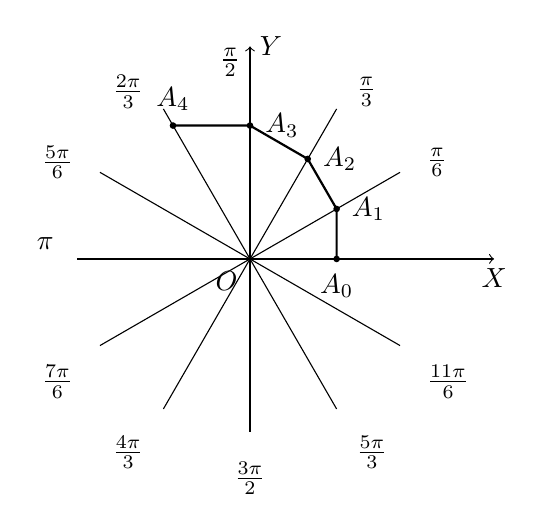
\begin{tikzpicture}[scale=1.0]
  % 十二条 30 度间隔射线
  \foreach \a in {0,30,...,330}{\draw[thin] (0,0)--(\a:2.2);}
  % 坐标轴
  \draw[->, thin] (0,0)--(3.1,0) node[below] {$X$};
  \draw[->, thin] (0,0)--(0,2.7) node[right] {$Y$};
  % 螺旋折线 A0-A1-A2-A3-A4（OA0=1 对应 1.1cm，公比 2/\sqrt{3}）
  \draw[thick] (1.1,0)--(1.1,0.635)--(0.733,1.270)--(0,1.694)--(-0.978,1.694);
  \fill (1.1,0) circle (1.2pt) node[below=2pt] {$A_0$};
  \fill (1.1,0.635) circle (1.2pt) node[right=2pt] {$A_1$};
  \fill (0.733,1.270) circle (1.2pt) node[right=2pt] {$A_2$};
  \fill (0,1.694) circle (1.2pt) node[right=2pt] {$A_3$};
  \fill (-0.978,1.694) circle (1.2pt) node[above=2pt] {$A_4$};
  \node[below left=1pt] at (0,0) {$O$};
  % 射线极角标注
  \node[right] at (30:2.45) {$\frac{\pi}{6}$};
  \node[right] at (60:2.45) {$\frac{\pi}{3}$};
  \node[left] at (90:2.5) {$\frac{\pi}{2}$};
  \node[left] at (120:2.45) {$\frac{2\pi}{3}$};
  \node[left] at (150:2.45) {$\frac{5\pi}{6}$};
  \node[above] at (180:2.6) {$\pi$};
  \node[below left] at (210:2.45) {$\frac{7\pi}{6}$};
  \node[below left] at (240:2.45) {$\frac{4\pi}{3}$};
  \node[below] at (270:2.45) {$\frac{3\pi}{2}$};
  \node[below right] at (300:2.45) {$\frac{5\pi}{3}$};
  \node[below right] at (330:2.45) {$\frac{11\pi}{6}$};
\end{tikzpicture}
